\documentclass[tikz,border=2pt]{standalone}
\usepackage{amsmath,amssymb}
\usepackage{tikz}
\usetikzlibrary{positioning}

\begin{document}
% Königsberg: four land areas and seven bridges become a multigraph with degrees 5, 3, 3, 3;
% all odd, so no closed walk crosses every bridge exactly once.
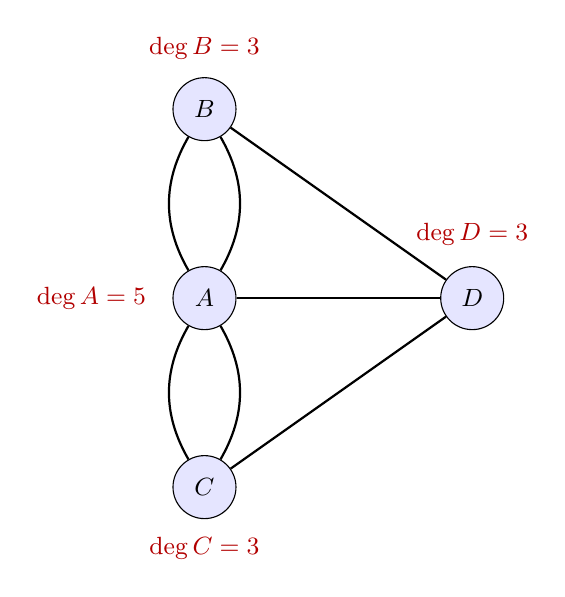
\begin{tikzpicture}[every node/.style={font=\small}, v/.style={draw, circle, fill=blue!10, minimum size=8mm, inner sep=0pt}]
	\node[v] (A) at (0,0) {$A$};
	\node[v] (B) at (0,2.4) {$B$};
	\node[v] (C) at (0,-2.4) {$C$};
	\node[v] (D) at (3.4,0) {$D$};
	\draw[thick] (A) to[bend left=30] (B);
	\draw[thick] (A) to[bend right=30] (B);
	\draw[thick] (A) to[bend left=30] (C);
	\draw[thick] (A) to[bend right=30] (C);
	\draw[thick] (A) -- (D);
	\draw[thick] (B) -- (D);
	\draw[thick] (C) -- (D);
	\node[red!70!black, left=6pt of A] {$\deg A=5$};
	\node[red!70!black, above=3pt of B] {$\deg B=3$};
	\node[red!70!black, below=3pt of C] {$\deg C=3$};
	\node[red!70!black, above=4pt of D] {$\deg D=3$};
	\end{tikzpicture}
\end{document}
